
\newcommand{\vdmkw}[1]{\texttt{\textbf{#1}}}
\chapter{Automatic Generation of Code}\label{sec:codegen}

It is possible to generate Java code\index{code generation} for a large subset of VDM-SL and VDM++ models.
%
In addition to Java, C and C++ code generators are currently being developed.
%
Both these code generators are in the early stages of development.
%
The C++ generator is not included with releases of Overture yet, but the C generator is far enough along that it can be included for testing purposes.
%
For comparison, code generation of VDM-SL and VDM++ specifications to both Java and C++ is a feature that is available in VDMTools~\cite{Java2VDMMan,CGMan,CGManPP}.
%
The majority of this chapter focuses solely on the Java code generator available in Overture, with a brief discussion of the C code generator ending the chapter.

\section{Use of the Java Code Generator}
\label{sec:javacg_use}

\begin{figure}[htbp]
\begin{center}
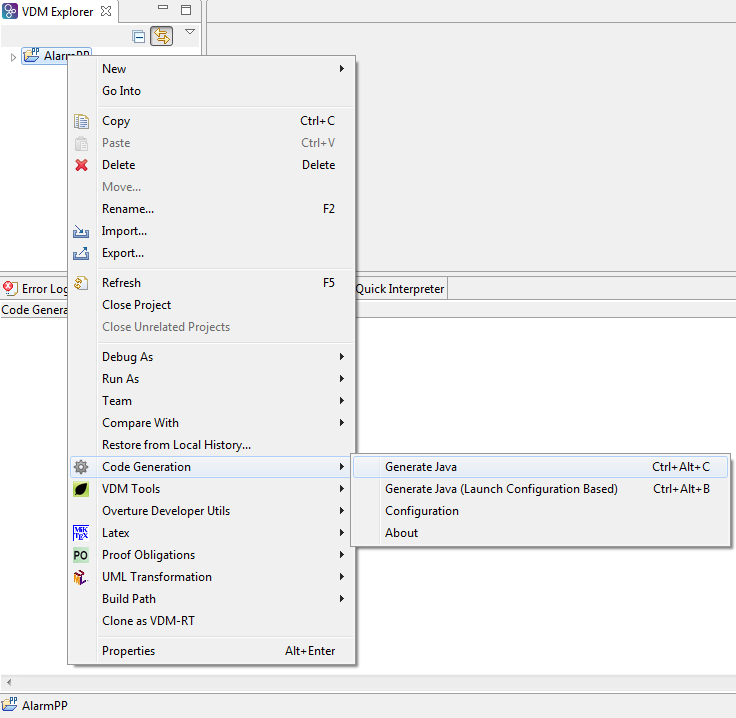
\includegraphics[width=10cm]{screenDumps/javacg_menu}
\caption{Launching the Java code generator.\label{fig:javacg_menu}}
\end{center}
\end{figure}

\begin{figure}[htbp]
\begin{center}
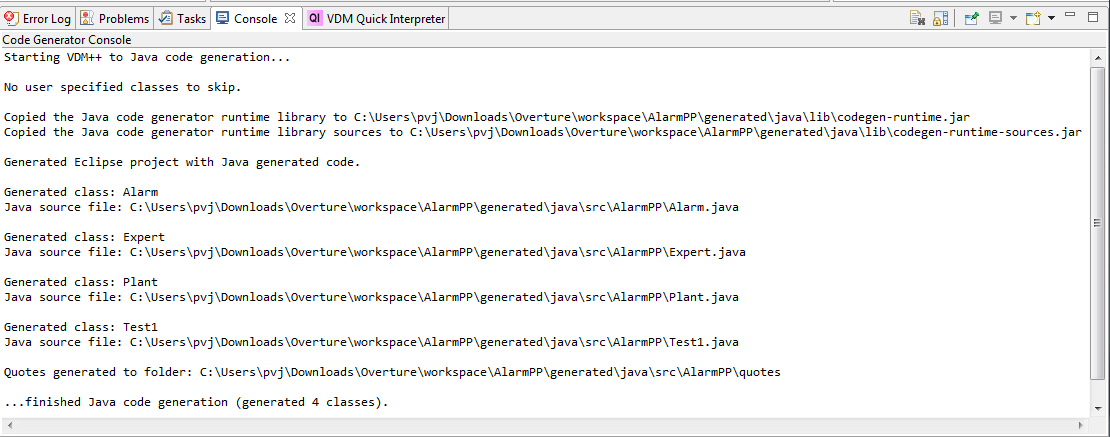
\includegraphics[width=\linewidth]{screenDumps/javacg_output}
\caption{The status of code generating the \texttt{AlarmPP}
example.\label{fig:javacg_output}}
\end{center}
\end{figure}

The Java code generator can be launched via the context menu as shown
in Figure~\ref{fig:javacg_menu}. Alternatively, this can be done by
highlighting the project in the VDM explorer and typing one of the
shortcuts associated to this plugin.\\

\noindent The Java code generator operates in two different modes:

\begin{itemize}

\item \emph{Regular mode:} In this mode the Java code generator
  produces an Eclipse project with all the generated code. Java code
  generation in this mode can also be initiated using the
  \texttt{Ctrl+Alt+C} shortcut.

\item \emph{Launch Configuration mode:}. Is currently limited to
  VDM++. This mode is like regular code generation except that the
  Java code generator also prompts the user for a launch configuration
  as input for the code generation process. Based on this launch
  configuration the Java code generator constructs an entry point (a
  \texttt{main} method really) that serves as an entry point for the
  generated code. Launch configuration based code generation can be
  initiated using the \texttt{Ctrl+Alt+B} shortcut.

\end{itemize}

\noindent Upon completion of the code generation process the status is
output to the console as shown in Figure~\ref{fig:javacg_output}. In
particular this figure shows the status of code generating the
\texttt{AlarmPP} model available in the Overture standard examples. As
indicated by the console output, the generated code is available as an
Eclipse project in the \texttt{<workspace>/<project>/generated/java}
folder.

\section{Configuration of the Java Code Generator}

The Java code generator can be configured via a preference page as
shown in Figure~\ref{fig:javacg_config}. The preference page can be
accessed in the way you would normally access an Eclipse preference
page or via the context menu shown above in
Figure~\ref{fig:javacg_menu}. The Java code generator provides a few
options that allows the user to configure the code generation process
(see Figure~\ref{fig:javacg_config}). The sub-sections below treat
each of these configuration parameters individually, in the order they
appear in the preference page.

\begin{figure}[htbp]
\begin{center}
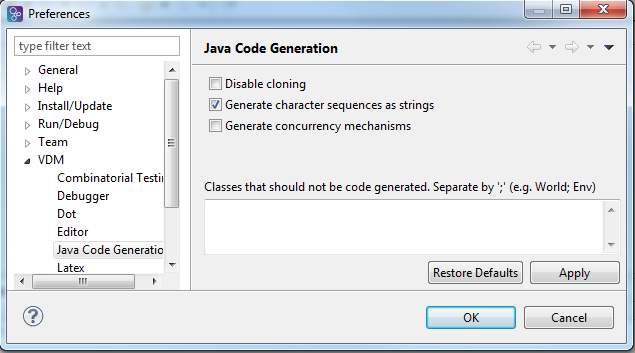
\includegraphics[width=15cm]{screenDumps/javacg_config}
\caption{Configuration of the Java code generator.\label{fig:javacg_config}}
\end{center}
\end{figure}

\subsection{Disable cloning}

In order to respect the value semantics of VDM the Java code generator
sometime needs to perform deep copying of objects that represent
composite value types (records, tuples, tokens, sets, sequences and
maps). For example, in VDM a record is a value type, which means that
occurrences of the record must be copied when it appears in the
right-hand side of an assignment, it is passed as an argument or
returned as a result. However, Java does not support composite value
types like structs and records, and as a consequence record types must
be represented using classes, which use reference semantics. This
means that an object reference, which is used to represent a composite
value type in the generated Java code must be deep copied when it
appears in the right-hand side of an assignment, it is passed as an
argument or returned as a result. For arbitrarily complex value types
(such as records composed of record or sets of composed of sets) deep
copying may introduce a significant overhead in the generated code. If
the specification subject to code generation does not truly rely on
value semantics the user may wish to disable deep copying of value
types in the generated code in order to remove this overhead. The user
should, however, be aware that disabling of cloning may lead to code
being generated that does not preserve the semantics of the input
specification and in general disabling of cloning is discouraged. By
default cloning is enabled.

\subsection{Generate character sequences as strings}
\label{sec:charseqs-as-strings}

In VDM a string is a sequence of characters and there is no notion of
a string type. Java in particular works differently since it uses a
separate type to represent a string. The default behaviour of the Java
code generator is to code generate sequences of characters as strings
and subsequently do the necessary conversion between between strings
and sequences in the generated code. Another possibility is to treat a
string literal for what it truly is, namely a sequence of characters,
and thereby avoid any conversion between strings and sequences. In
order to do that, i.e.\ \textit{not} generating character sequences as
strings, the corresponding option must be unchecked.

\subsection{Generate concurrency mechanisms}

If the user does not rely on the concurrency mechanisms of VDM++ and
does not want to include support for them in the generated code the
corresponding option in the preference page must be unchecked. By
default the behaviour of the Java code generator is to not include
support for the concurrency mechanisms of VDM++ in the generated code.

\subsection{Generate Java Modeling Language (JML) annotations}

When a VDM model is code generated to Java all the contract-based
elements of the model, i.e.\ the pre conditions, post conditions and
invariants, are ignored by default. When this option is selected the
contract-based elements of a VDM-SL model are translated to JML
annotations~\cite{Burdy&05} that are added to the generated Java
code. This allows the system properties, expressed in terms of pre
conditions, post conditions and invariants, to be checked against the
generated code. The generated JML annotated programs can be checked
for corrected using a JML tool such as
OpenJML\footnote{\url{http://www.openjml.org}}.\\

\subsection{Use JML \textbackslash invariant\_for to explicitly check record invariants}
\label{sec:inv-for}

The JML generator offers two ways to perform the invariant check of a
record. By default the JML generator does this by invoking a
\texttt{valid} method generated for each record definition. When this
option is enabled the JML generator instead uses the JML
\vdmkw{invariant\_for} construct to perform the record invariant
checks. Note that the \vdmkw{invariant\_for} construct is currently
not supported by OpenJML, which is the reason why this option is not
enabled by default.

\subsection{Generate VDM location information for code generated constructs}
\label{sec:vdm-loc}

When a VDM model is code generated it can be helpful to know where the
constructs in the generated code originate from. When this option is
enabled the Java code generator will generate VDM location information
for methods, statements and local declarations in the generated
code. More specifically, the Java code generator will generate a Java
source code comment containing the name of the VDM source file and the
line number and the position, for each method, statement and local
declaration. As an example, the code fragment below says that the Java
return statement originates from a VDM construct at line 25,
position 12 in \texttt{File.vdmsl}.\\

\noindent \texttt{/* File.vdmsl 25:12 */\\return 42;}

\subsection{Choose output package}
\label{sec:javapackage}

The Java code generator allows the output package of the generated
code to be specified. If the user does not specify a package, the code
generator outputs the generated Java code to a package with the same
name as the VDM project. If the name of the project is not a valid
java package, then the generated code is output to the default Java
package.

\subsection{Skip classes/modules during the code generation process}

It may not always make sense to code generate every class or module in
a VDM project. A class or module can often be skipped if it acts as an
execution entry point or it is used to load input for the
specification. Classes or modules that the user wants to skip can be
specified in the text box in the Java code generator preference page
by separating the class/module names by a semicolon. As an example,
\texttt{World;Env} makes the code generator skip code generation of
\texttt{World} and \texttt{Env}, while generating code for any other
module or class. For convenience the output of the Java code generator
will also inform the user about what classes or modules are being
skipped.

\section{Limitations of the Java Code Generator}

If the Java code generator encounters a construct that it cannot code
generate it will report it as unsupported to the user and the user can
then try to rewrite that part of the specification using other
(supported) constructs. Reporting of unsupported constructs is done
via the console output and using editor markers. In order to
demonstrate this, Figure~\ref{fig:javacg_unsupported} shows the
console output of the Java code generator when it encounters a type
bind, which is an example of an unsupported language construct. Note
the small marker appearing in the editor in order to point out where
use of the construct appears. For the type bind example in
Figure~\ref{fig:javacg_unsupported} the following message is reported:\\

\noindent \texttt{Following VDM constructs are not supported by the
  code generator:\\ b:(bool * bool) (ATypeMultipleBind) at
  6:14. Reason:\\ Type binds are not supported}\\

\begin{figure}[htbp]
\begin{center}
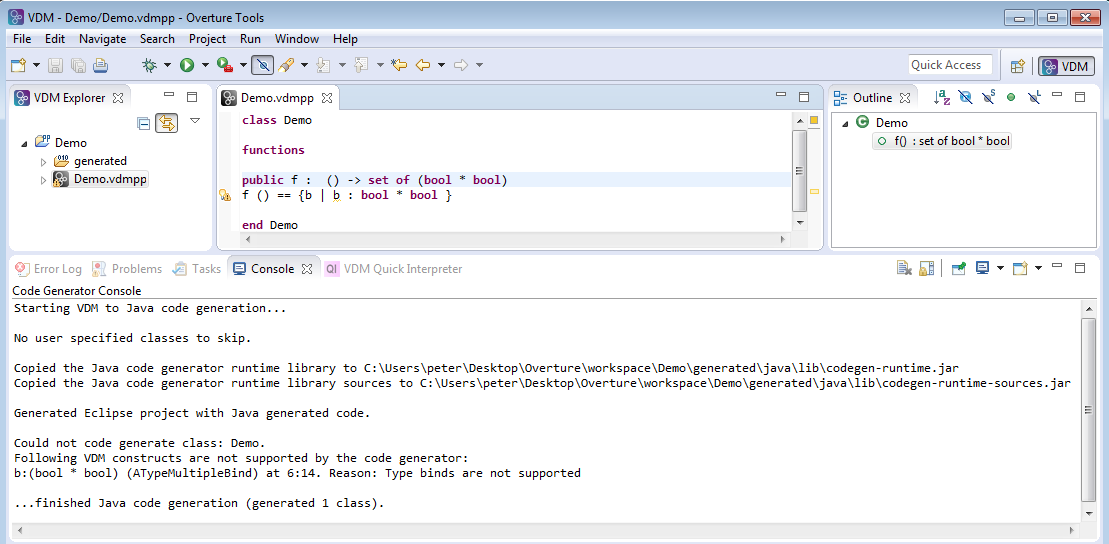
\includegraphics[width=\linewidth]{screenDumps/javacg_unsupported}
\caption{Reporting of unsupported constructs in the
console.\label{fig:javacg_unsupported}}
\end{center}
\end{figure}

The user will get similar messages and markers for other unsupported
VDM constructs. To summarise, the Java code generator currently does
not support code generation of multiple inheritance and neither does
it support traces, type binds, invariant checks and pre and post
conditions. Furthermore, let expressions appearing on the right-hand
side of an assignment will also be reported as unsupported. The Java
code generator also does not support every pattern. The patterns that
are currently not supported are: object, map union, map, union, set,
sequence, concatenation and match value.

\section{The Code Generation Runtime Library}

The generated code relies on a runtime library used to represent some
of the types available in VDM (tokens, tuples etc.) as well as
collections and support for some of the complex operators such as
sequence modifications. For simplicity every Eclipse project generated
by the Java code generator contains the runtime library. More
specifically, there is a copy of the runtime library containing only
the binaries (\texttt{lib/codegen-runtime.jar}) as well as a version
of the runtime library that has the source code attached
(\texttt{lib/codegen-runtime-sources.jar}). The runtime library is
imported by every code generated class using the Java import statement
\texttt{\textbf{import} org.overture.codegen.runtime.*;} and in order
to compile the generated Java code the runtime library must be visible
to the Java compiler.

Similar to VDMTools the runtime library also provides implementation
for subset of the functionality available in the standard libraries:
The runtime library provides a full implementation of the
\texttt{MATH} library, support for conversion of values into character
sequences as provided by the \texttt{VDMUtil}, and finally
functionality to write to the console as available in the \texttt{IO}
library.

\section{Translation of the VDM types and type constructors}
\label{sec:type-mappings}

Table ~\ref{tbl:type-mappings} describes how the VDM type(s) in the
left column are represented in the generated Java code (the right
column). In this table \texttt{pack} is the user-specified root
package of the generated Java code (see section \ref{sec:javapackage})
and \texttt{E}, \texttt{D} and \texttt{R} represent arbitrary VDM
types. The type mapping in the last row is only used when the
\emph{Generate character sequences as strings} option is selected (see
section \ref{sec:charseqs-as-strings}). Some of the types used to
represent the VDM types are native Java types (from package
\texttt{java.lang}), others are part of the Java code generator
runtime library (from package \texttt{org.overture.codegen.runtime}),
and some are generated.

\begin{center}
    \begin{tabular}{| l | l |}
    \hline
    VDM type(s) & Java type \\ \hline
    \vdmkw{bool} & \texttt{java.lang.Boolean} \\ \hline
    \vdmkw{nat}, \vdmkw{nat1}, \vdmkw{int}, \vdmkw{rat}, \vdmkw{real} & \texttt{java.lang.Number} \\ \hline
    \vdmkw{char} & \texttt{java.lang.Character} \\ \hline
    \vdmkw{token} & \texttt{org.overture.codegen.runtime.Token} \\ \hline
    Tuple types (e.g.\ \vdmkw{nat} \texttt{*} \vdmkw{nat}) & \texttt{org.overture.codegen.runtime.Tuple} \\ \hline
    Union types (e.g.\ \vdmkw{nat} \texttt{|} \vdmkw{nat}) & \texttt{java.lang.Object} \\ \hline
    Quote type \texttt{ <T>} & \texttt{pack.quotes.TQuote} \\ \hline
    User-defined types \texttt{T = D} & Represented using the representation of type \texttt{D} \\ \hline
    A class \texttt{C} & \texttt{pack.C} \\ \hline
    Record type \texttt{R} defined in class or module \texttt{M} & Inner class \texttt{pack.M.R}  \\ \hline
    \vdmkw{set of} \texttt{ E} & \texttt{org.overture.codegen.runtime.VDMSet} \\  \hline
    \vdmkw{map} \texttt{ D } \vdmkw{to} \texttt{ R}, \vdmkw{inmap} \texttt{ D } \vdmkw{to} \texttt{ R} & \texttt{org.overture.codegen.runtime.VDMMap} \\  \hline
    \vdmkw{seq of} \texttt{ E}, \vdmkw{seq1 of} \texttt{ E}  & \texttt{org.overture.codegen.runtime.VDMSeq} \\  \hline
    \vdmkw{seq of char}, \vdmkw{seq1 of char} & \texttt{java.lang.String} \\  \hline
    \end{tabular}
  \captionof{table}{The type mappings used by the Java code generator.}
  \label{tbl:type-mappings}
\end{center}
%
%
%
\section{The C Code Generator}
Translation of VDM models to C code is a new feature of Overture.
%
The target language of the C generator is the executable subset of VDM-RT.
%
It is not yet feature-complete, but it can handle models which do not use sophisticated features of VDM-RT.
%
The following list describes the current state of language feature support.
%
Items in black are tested and known, to the best of the developers' knowledge, to translate correctly to C.
%
Items in \textcolor{red}{red} are not yet supported.
%
%
%
\begin{itemize}
%
\item  Classes.
%
\item  Inheritance.
%
\item  Overriding.
%
\item  Type definitions.
\begin{itemize}
\item  \textcolor{red}{Type invariants}.
\end{itemize}
%
\item  Boolean and numeric expressions.
\begin{itemize}
\item  \textcolor{red}{Quantifiers}.
\end{itemize}
%
\item  \textcolor{red}{Products}.
%
\item  Sets, sequences and maps.
\begin{itemize}
\item  \textcolor{red}{Nested state designators, \emph{e.\@g.\@} \texttt{a(i)(j) := k}}.
\end{itemize}
%
\item  Explicit functions and operations.
\begin{itemize}
\item  \textcolor{red}{Lambda abstractions}.
\item  \textcolor{red}{Pre-\@ and post-conditions}.
\end{itemize}
%
\item  Loops.
\begin{itemize}
\item  \textcolor{red}{For index loops}.
\item  \textcolor{red}{While loops}.
\end{itemize}

%
\item  \textcolor{red}{Real-time and distribution features}.
\begin{itemize}
\item  The \verb|time| statement.
\end{itemize}
%
\item  I/O library.
\begin{itemize}
\item  \textcolor{red}{String patterns}.
\item  \textcolor{red}{File I/O}.
\end{itemize}
%
\item MATH library.
\begin{itemize}
\item  \textcolor{red}{exp()}
\item  \textcolor{red}{acot()}
\item  \textcolor{red}{acos()}
\item  \textcolor{red}{asin()}
\item  \textcolor{red}{cot()}
\item  \textcolor{red}{tan()}
\item  \textcolor{red}{cos()}
\item  \textcolor{red}{rand()}
\item  \textcolor{red}{srand()}
\item  \textcolor{red}{srand2()}
\end{itemize}
%
\end{itemize}

Like the Java code generator, the C code generator can be invoked from the context menu in the VDM project explorer.
%
Unlike the Java code generator, it must be installed through Overture's ``Install New Software \dots'' feature.
%
The repository URL is
%
%
%
\begin{quote}
\url{http://overture.au.dk/vdm2c/master/repository/}.
\end{quote}
%
Code is emitted to the folder \texttt{generated/src/c} under the corresponding VDM project.
%
Please note that this folder is wiped clean each time code is generated.
%
Additional development work on the generated code \emph{must not} be carried out in this folder.
%%% Local Variables:
%%% mode: latex
%%% TeX-master: "../OvertureIDEUserGuide"
%%% End:
